\documentclass[11pt]{article}
\usepackage[english]{babel}
\usepackage{natbib}
\usepackage{url}
\usepackage[utf8x]{inputenc}
\usepackage{amsmath}
\usepackage{graphicx}
\graphicspath{{images/}}
\usepackage{parskip}
\usepackage{fancyhdr}
\usepackage{vmargin}
\setcitestyle{square}
\setmarginsrb{3 cm}{2.5 cm}{3 cm}{2.5 cm}{1 cm}{0.75 cm}{1 cm}{1.5 cm}
\usepackage[justification=centering]{caption}
\title{Spark Ignited Automobile Engines}								% Title
										% Date

\makeatletter
\let\thetitle\@title
\let\theauthor\@author
\let\thedate\@date
\makeatother

\pagestyle{fancy}
\fancyhf{}
\rhead{\theauthor}
\lhead{\thetitle}
\cfoot{\thepage}

\begin{document}

%%%%%%%%%%%%%%%%%%%%%%%%%%%%%%%%%%%%%%%%%%%%%%%%%%%%%%%%%%%%%%%%%%%%%%%%%%%%%%%%%%%%%%%%%

\begin{titlepage}
	\centering
    \vspace*{0.5 cm}
    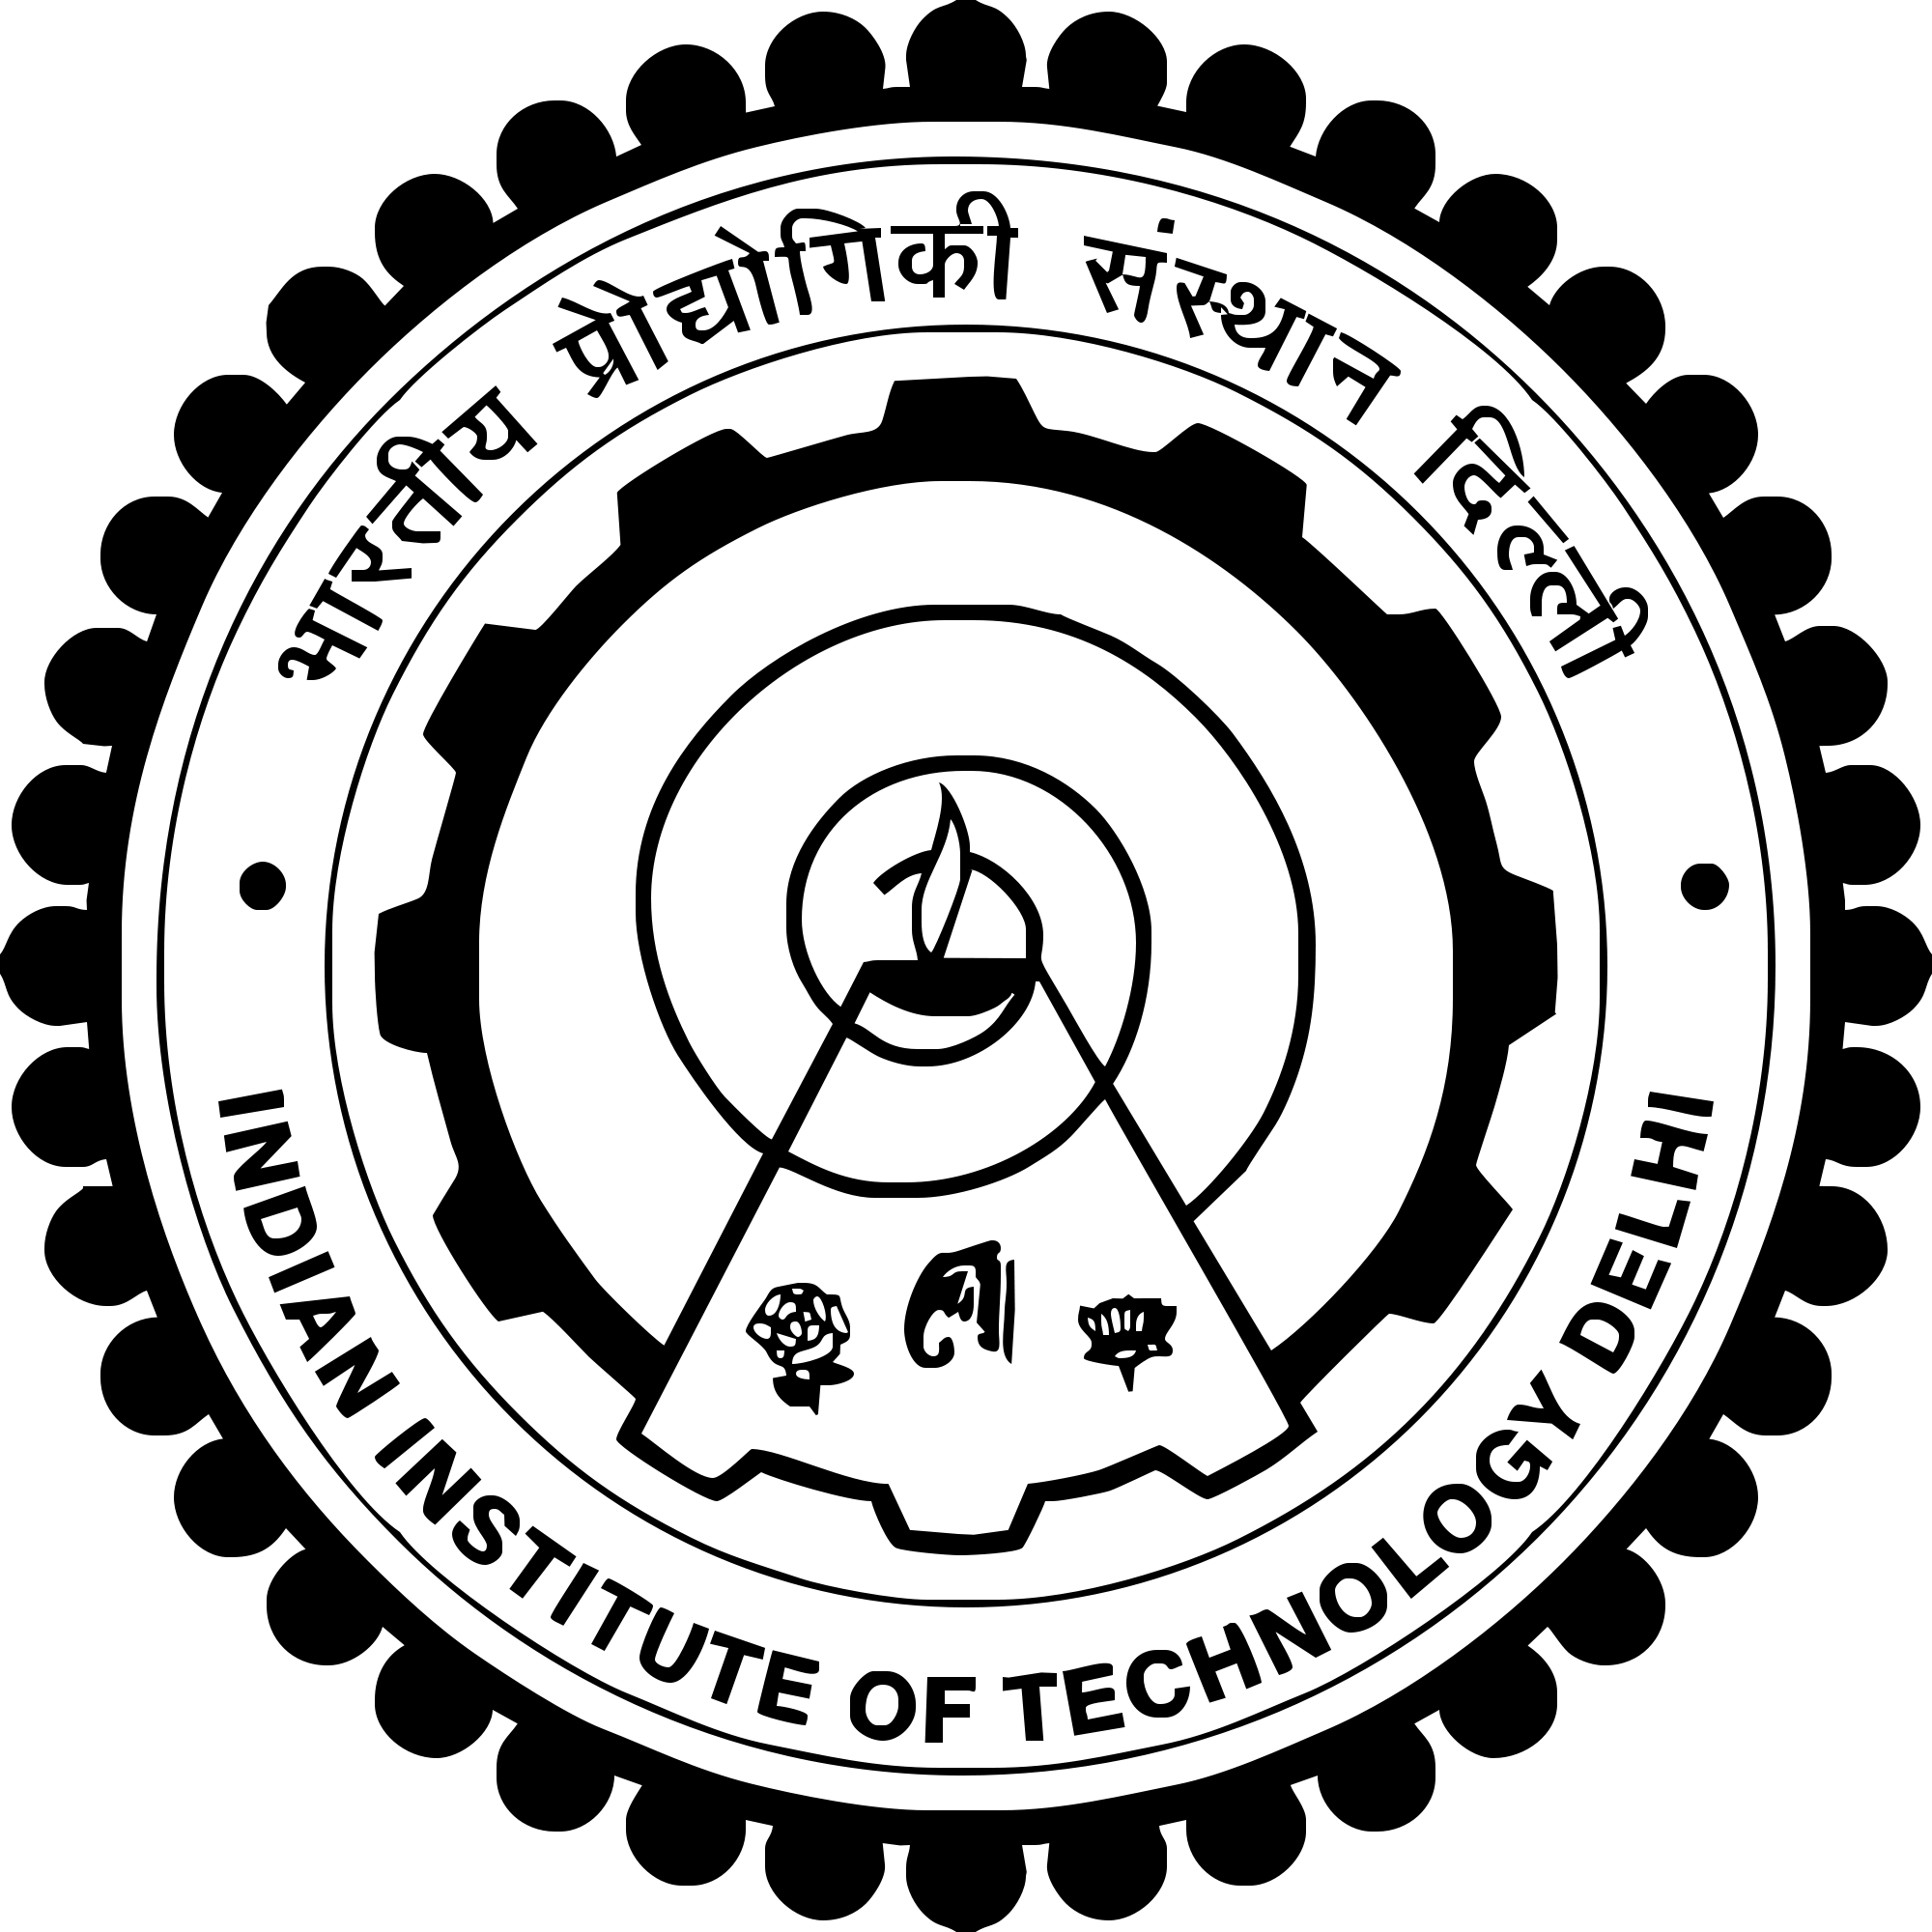
\includegraphics[scale = 0.075]{IIT_Delhi_logo.png}\\[1.0 cm]	% University Logo
    \textsc{\LARGE Indian Institute of Technology Delhi}\\[2.0 cm]	% University Name
	\textsc{\LARGE MCL142 Term Paper}\\[0.5 cm]				% Course Code
	\rule{\linewidth}{0.2 mm} \\[0.4 cm]
	{ \huge \bfseries \thetitle}\\
	\rule{\linewidth}{0.2 mm} \\[3.5 cm]
	
	\begin{minipage}{0.4\textwidth}
		\begin{flushleft} \large
			\emph{Submitted To:}\\
			Dr. M.R. Ravi\\
			Professor\\
			Mechanical Engg. Dept.\\
			IIT Delhi
			\end{flushleft}
			\end{minipage}~
			\begin{minipage}{0.4\textwidth}
            
			\begin{flushright} \large
			\emph{Submitted By :} \\
			Hritik Bansal\\
			(2016EE10071)\\
			Gantavya Bhatt\\
			(2016EE10694)\\
			Anubhav Bhatia\\
			(2016EE10835)\\
		\end{flushright}
        
	\end{minipage}\\[2 cm]
	
\end{titlepage}

%%%%%%%%%%%%%%%%%%%%%%%%%%%%%%%%%%%%%%%%%%%%%%%%%%%%%%%%%%%%%%%%%%%%%%%%%%%%%%%%%%%%%%%%%

\tableofcontents
\pagebreak
%figure1 ka reference-> https://www.researchgate.net/figure/Four-stroke-cycle-for-spark-ignition-engines-Wikipedia-2014_fig15_284950622
% Book
% 
%%%%%%%%%%%%%%%%%%%%%%%%%%%%%%%%%%%%%%%%%%%%%%%%%%%%%%%%%%%%%%%%%%%%%%%%%%%%%%%%%%%%%%%%%
\begin{center}
    \section*{Abstract}
The study of different kind of engines used in automobiles is of prime importance in thermodynamics. Their behaviour defines the efficiency and power output of the automobiles that we use in day-to-day life. This paper particularly focuses on the spark ignited automobile engines. However, the width and depth of this topic restricts us to highlight the most notable aspects of this kind of engine. We shall cover topics like historical development of these engines followed by their classification based on their mechanics and design. We shall look at the thermodynamic aspect involved in these kind of engines. This helps us to reason their observed traits,and differences with the counterparts. Last section shall give a brief idea about the contribution of every author followed by the acknowledging the references.   


\end{center}
\section{Historical Development of Engines}
The very initial engines that were developed were not the ignition engines but they involved steam. One of the early successful engines developed were the Newcomen engine that use to operate by condensing the steam and thereby creating the vacuum leading the atmosphere to do the compression work. This compression work was used to pump out the water. Later on as the time progressed their was a significant improvement in terms of the fuel efficiency and the power output. \cite{ref15}\\
 Four-stroke Otto cycle based engine came into existence in 1869 after its invention by Nikolaus August Otto, a German engineer in 1867.These otto engine are so effective that they are in use currently in the transportation .Diesel engine developed by Rudolph Diesel, another German engineer were much heavier and powerful than gasoline engines. Since that time, the advancements happened by changing the design of the engine to reduce the friction, but the principle remained more or less the same. We will see in the subsequent sections that what were the different possible designs, the involved processes and the thermodynamics involved in the process.
\section{Classifying Engines on the basis of their Mechanics}
\begin{flushleft}
The first basis of classification of the Spark Ignited engine can be done on the basis of their mechanics. So, on this basis, we can can divide them into the reciprocating type engines and the rotary engines.
\end{flushleft}
\subsection{Reciprocating type engines}
As the name suggests, reciprocating type engines consists of a moving part that moves in a rectilinear fashion. This moving part is called a \textit{piston}. The piston moves in the up-down motion and its translation motion is converted to a rotational motion with the help of a crankshaft. That is why reciprocating engines are also called as piston engines. This piston sits inside a cylinder inside which it performs the rectilinear motion. The basic cylinder-piston is illustrated in Figure[1]. \\

\begin{flushleft}
Based on the extreme positions of the piston inside the cylinder, we define the following terminologies:- \\[-0.2in]
\subsubsection{Top Dead Center}
Though a cylinder can be in any position, we define it as the location of the piston when the volume of the cylinder is minimum, or going by the figure mentioned above, its the topmost point to which the piston reciprocates.

\begin{center}
        \begin{figure}[h]
        \centering
          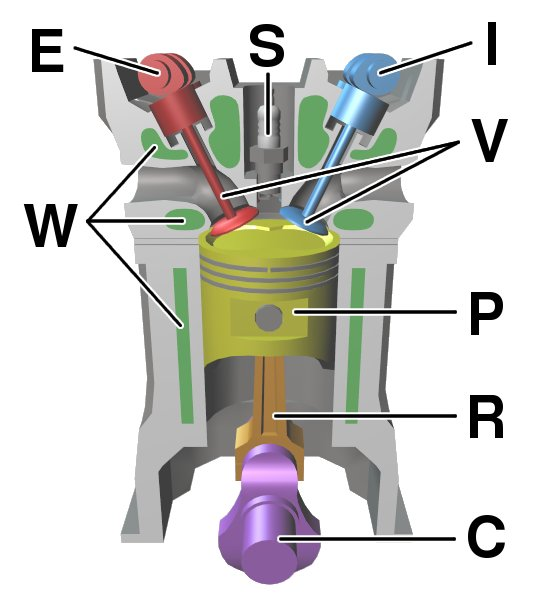
\includegraphics[width=100mm, height=100mm]{piston.jpg}
          \caption{Piston, C. Crankshaft E. Exhaust camshaft I. Intake camshaft P. Piston R. Connecting rod S. Spark plug W. Water jacket for coolant flow V. Valves\\ (Image courtesy \cite{ref9})
          }
          \label{fig:Piston}
        \end{figure}
\end{center}

\subsubsection{Bottom Dead Center}
Bottom dead center is defined in the same way as we defined the top dead center, as the point when the volume of the cylinder is maximum, or by the figure mentioned above, its the bottom-most point to which the piston reciprocates.
\subsubsection{Combination of cylinders}
To output high power and torque, especially for high power vehicles such as cars, trucks, etc. single cylinder is never used. Thus the cylinders are used in a combination to add their power output. Their spatial arrangement leads us to the different type of configurations available - \\
\textbf{1) Inline Engine:\\}
The first idea that comes into mind to ensemble the power output of each cylinder piston arrangement is the straight line connection.So, as the name suggests, the inline engine connects the piston in the straight line in the configuration similar to the figure shown below. An inline engine is used with 2, 3, 4, 5, 6 or up to 8 cylinders.\\
\end{flushleft}
\begin{center}
        \begin{figure}[!h]
        \centering
          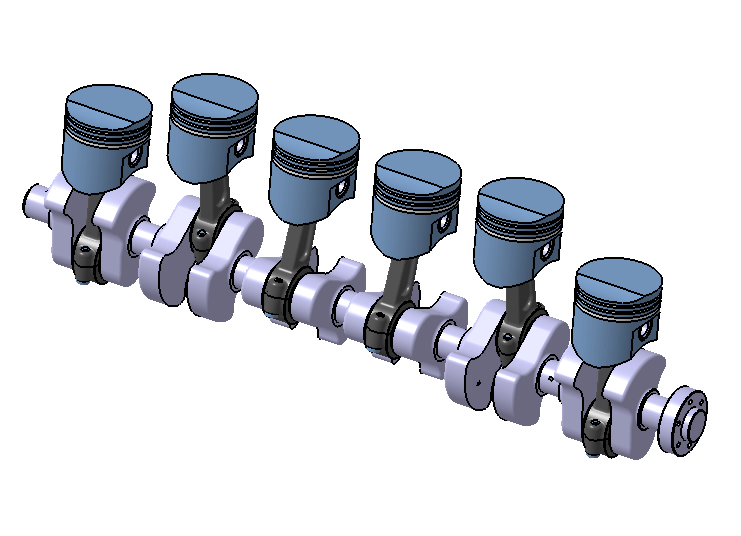
\includegraphics[width=50mm, height=50mm]{Inline.jpg}
          \caption{An Inline piston combination. Here only pistons are shown without the cylinders\\ (Image courtesy \cite{ref11})
          }
          \label{fig:Piston}
        \end{figure}
\end{center}
\begin{flushleft}
\textbf{2) V\_shape Engine: \\}
Soon after the development of the inline engine, to produce more power output by surpassing the spatial constraints in the inline engine, people came with the idea of connecting the 2 cylinders in an angle. This arrangement is similar to the alphabet 'V' by connecting the two banks of cylinders side-by-side.Generally, this arrangement is used with 6, 8, 10, 12 cylinder piston configuration.
\end{flushleft}
\begin{center}
        \begin{figure}[!h]
        \centering
          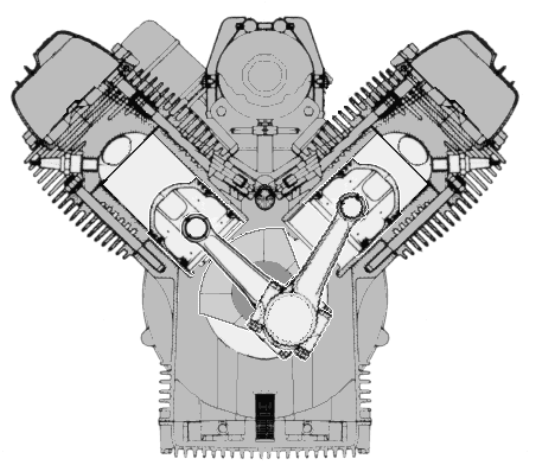
\includegraphics[width=50mm, height=50mm]{V_shape.PNG}
          \caption{A cross section of a V-shape engine\\ (Image courtesy \cite{ref10})
          }
          \label{fig:Piston}
        \end{figure}
\end{center}
\begin{flushleft}
\pagebreak
\textbf{3) W-shaped Engine : \\}
The motivation for developing this engine is similar to that of the V shape engines. In V shape we have 2 cylinder piston in a plane at a relative angle, here on the other hand we have 3 cylinder pistons in a plane with angles displaced to each other. These are generally used in high power sports car. The number of cylinders go even up to 18 in this configuration. 
\end{flushleft}

        \begin{figure}[!h]
        \centering
          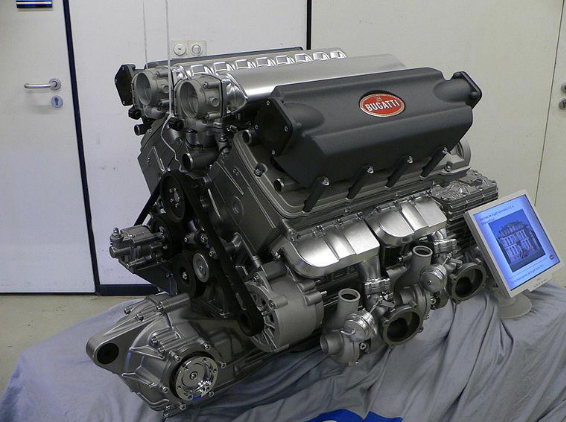
\includegraphics[width=50mm, height=50mm]{W_shape.PNG}
          \caption{A W16 engine in Buggati Veyron\\ (Image courtesy \cite{ref12})
          }
          \label{fig:Piston}
        \end{figure}

\subsection{Rotary Type Engine}
These engine lack any kind of Reciprocating motion and rotate so that to rotate the final shaft. It consisted of odd number of cylinders per row in a radial fashion with stationary crankshaft. It was efficient in terms of the conversion of power as they do not have the translation motion. We will discuss the limitations in the subsequent sections. Following is one of the basic design of a rotary based engine.\\

\begin{center}
        \begin{figure}[!h]
        \centering
          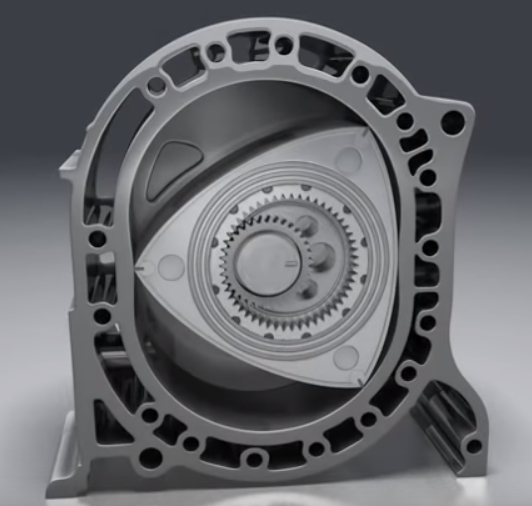
\includegraphics[width=60mm, height=60mm]{rotary.PNG}
          \caption{Cross section of a rotary type engine\\ (Image courtesy \cite{ref13})
          }
          \label{fig:Piston}
        \end{figure}
\end{center}

\textbf{\textit{What does cc in the engine specification sheet means?}}\\
As we all know, while buying a vehicle we see the engine specification of that vehicle, there we can see the term 'cc'. Its actually a measure of the volume of the cylinder of the engine. Mathematically it can be said to be equal to  \(V_{BDC}-V_{TDC}\). So does it tells us the power of the engine? Indeed the power output of an engine depends on the compression ratio, but it depends on the other parameters as well. For example, current formula 1 engines, they have 1600cc and produce around 800 - 1000 horsepower, however a 1600cc engine from a VW beetle produces about 50 horsepower, a massive difference.

\section{Typical SI Engine Designs}

The typical designs of typical SI engines can be broadly categorized into Four Stroke Engines and Two Stroke Engines. We shall have a look at them in this section. Also, we will have a passing mention about the rotary type SI engines and at the end, we will present a brief comparison between these designs as their pros and cons.

\subsection{Four Stroke Engine}
Most of the spark ignition engines have a piston which executes four complete strokes and a crankshaft which completes two complete revolutions(${720^0}$) in each cycle. Each stroke of a four-stroke engine performs a particular thermodynamic process. Four Stroke engine completes Intake, Compression, Ignition, 
Power and Exhaust strokes.
 A brief overview of the Design of the four-stroke SI engine can be seen in Figure[1].\\


\begin{figure}[!h]
  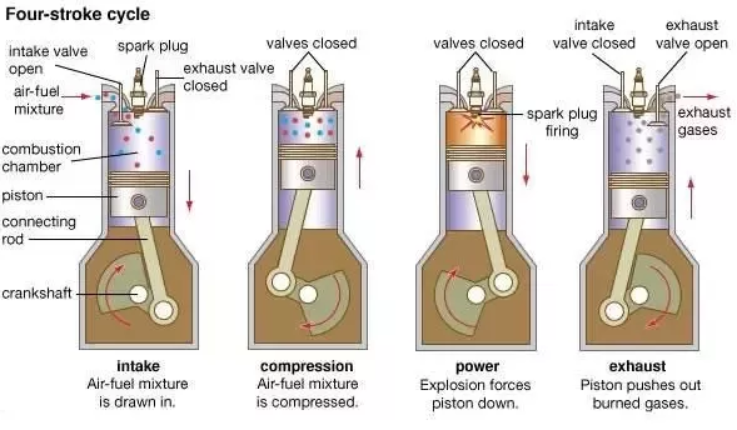
\includegraphics[width=\linewidth,scale=0.75]{FourStroke.png}
  \caption{Four Stroke Spark Ignition Engine Design(Image courtesy \cite{fig1})}
  \label{fig:Four Stroke Spark Ignition Engine Design}
\end{figure}

\textbf{Intake:} Air-fuel mixture enters the combustion chamber through the intake valve such that the piston moves from TDC to BDC. This piston movement creates a low-pressure area, and atmospheric pressure takes air-fuel mixture through the intake valve. The valve closes so that air-fuel mixture gets sealed inside the combustion chamber \cite{ref2}.

\textbf{Compression Stroke:} This stroke involves the compression of Air-fuel mixture from BDC to TDC by the piston. The amount of energy released by the mixture volume depends upon the pressure up to which it is compressed. The compression work done by the piston is stored as heat in the air-fuel mixture which in turn increases its temperature. The amount of work produced from the ignition of this compressed mixture is much more than the work required to compress it till TDC, which makes it pretty efficient \cite{ref2}.\\
We define a quantity Static compression ratio in regards to Compression Stroke as:
\[CR=\frac{V_d+V_c}{V_c}\] where ${V_c}$ is the smallest capacity of the combustion chamber also known as the clearance volume and
$V_d$ is the amount of the displacement when the piston goes from its lowermost position in the chamber to the topmost position \cite{ref3}. The fuel efficiency of a Spark-Ignition Engine increases with an increase in compression ratio. However, a large value of compression ratio implies a larger operator effort to start the engine \cite{ref2}.

\textbf{Ignition:} Oxidization of compressed air-fuel mixture happens in this event. The ignition is caused due to the spark plug at the top of the combustion chamber comes in contact with the fuel-air mixture. The flame progresses through the chamber until the entire mixture gets burnt \cite{ref2}. 

\textbf{Power Stroke:} As the combustion of the mixture happens in a closed volume, the temperature inside the chamber increases rapidly. The increase in temperature of the exhaust gases and residual air leads to the development of high pressure inside it following the ideal gas law. These gases apply high pressure on the piston which is in turn connected to the crankshaft(in Figure[1]). This work done by the gases is used for rotating the shaft, propulsion, and aiding the compression stroke of nearby cylinders. \cite{ref4}. 

\textbf{Exhaust:} At the end of the power cycle, combustion by-products remain in the combustion chamber at lower temperatures. The evacuation of the exhaust gases to the atmosphere is achieved by the piston movement from BDC to TDC through exit valve \cite{ref2}. This makes the spark ignition engine ready for the next four-stroke cycle.\\
Though the 4 stroke engine has come out to be the most success full of all of the engines designs, it still has some of the \textbf{\emph{disadvantage}} -\\ 
\textit{\textbf{Since the fuel is burnt in every 2 rotations that is 4 strokes, the power delivered is relatively less per rotation if we were to compare this with the 2 stroke variant of the reciprocating engines. }}
\subsection{Two Stroke Engine}

In this engine, as the name suggests there is one complete revolution of the crankshaft in one cycle as opposed to two, in four stroke engine. All the four functions described above are performed in just two strokes viz. Power and Compression Stroke \cite{ref5}. Figure[2] illustrates the two strokes involved in these kinds of engines.\\
Intake and Exit valves are replaced by displaced openings in case of two-stroke engines as shown in Figure[2]. Upstroke event is similar to the compression stroke of four-stroke engine where air-fuel mixture is compressed to slightly higher pressure. The mixture is spark ignited as explained earlier. However, during the downstroke phase, the piston uncovers the exit valve through which exhaust can pass out. In addition to this, the fresh air-fuel mixture is added to the combustion chamber simultaneously. This implies the intake; exhaust event happens along with the pressure stroke in the case of the two-stroke engine. Interestingly, a typical compression ratio of a two-stroke engine is similar to that of four-stroke engine.
\textbf{Some disadvantages of 2 Stroke engine}\\
\textbf{1)}Logically, the efficiency of the two-stroke engine is less than that of four-stroke engine. This is because some of the fresh air-fuel mixture gets removed during the pressure stroke along with the exhaust gases.  \\
\textbf{2)}Since the fuel is consumed in every cycle or in every second stroke, the fuel consumption is much more as compared to the 4-stroke engine. This makes the engine less fuel efficient although it results in uniform power delivery.

\begin{figure}[!h]
  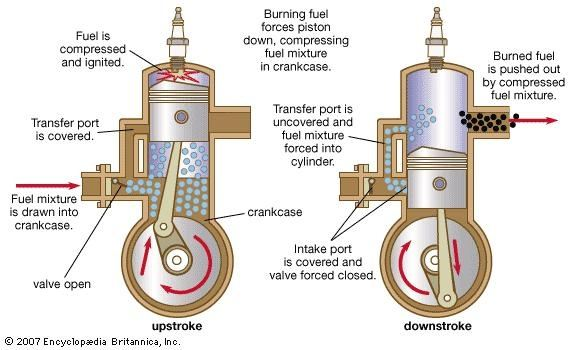
\includegraphics[width=\linewidth,scale=0.75]{2strokeEngine.jpg}
  \caption{Two Stroke Spark Ignition Engine Design}
  \label{fig:Two Stroke Spark Ignition Engine Design}
\end{figure}
In spite of the fact that they are known to have higher pressure-to-weight ratios which make them suitable to be used in small size, weight applications like motorcycles etc. \cite{ref5}, they have many disadvantages\\



\subsection{Wankel Engine}

Wankel Engine converts the pressure to the rotary motion directly rather than using a linear piston arrangement in four/two-stroke engines. It is also based on four-step process: Intake, Compression, Spark and Exhaust \cite{ref7}.\\
Rotating rotor instead of the crankshaft is one of the most components of this engine. In the intake process, the air-fuel mixture is drawn due to the decrease in the pressure caused by the rotating rotor. The sides of the rotor touch the housing such that the fuel in one cycle does not mix with the other. The rotor forces the mixture into a tighter area in the compression process. In this process, the air-fuel mixture is brought at the correct pressure required for ignition. This high-pressure mixture is ignited in the next stage with a spark plug leading to the release of a high amount of heat and exhaust gases. The heat released will be used to rotate the rotor, and it is the effective work extracted from one complete revolution of the rotor. Exhaust gases thus formed are taken out of this system through exhaust outlet \cite{ref7}. Figure[3] encapsulates this discussion pretty clearly.

\begin{figure}[h]
  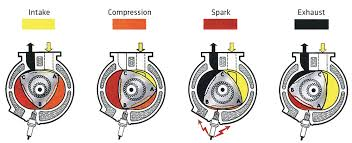
\includegraphics[width=\linewidth,scale=0.75]{wankel.jpg}
  \caption{Wankel Spark Ignition Engine Design(Image courtesy \cite{ref7})}
  \label{fig:Wankel Spark Ignition Engine Design}
\end{figure}
Wankel engine has the continous rotational motion, thus the torque produced by it is more uniform as compared to any reciprocating engine. But even though it directly converts the pressure into the rotary motion, it has many drawbacks limiting its application making it an obsolete tech. Some are as follows - \\
\textbf{1)}
The Wankel engine has comparatively lower fuel efficiency and emissions \cite{ref8}. They generally suffer a lot of wear tear as the design demands that the rotor should touch the housing at all times \cite{ref7}. \\
\textbf{2)}Unlike a piston engine in which the gas sealing surfaces (piston rings) are lubricated by the oil control ring during the reciprocating movement, the rotary engine’s need much more lubrication for its smooth rotary motion. Thus its sealing surfaces are cooled \& lubricated by introducing engine oil into the combustion chamber (via the Oil Metering System). This has some drawbacks because motor oils do not burn clean, resulting in increased residue buildup in the engine, which has to be cleaned time to time.

\section{Introduction to Ideal Otto Cycle}
The Otto cycle is a cycle which describes the series of processes used in spark ignition internal combustion engines for example Four Stroke Engine and Two Stroke Engine. As discussed in previous section that these engines have a piston which executes four complete strokes namely Intake Stroke, Compression Stroke, Ignition, Power Stroke and Exhaust Stroke. The PV diagram for the cycle \cite{ref14} is shown in figure below. Different processes of Otto Cycle as follows: 
\newline
\textbf{1)} Intake stroke, where fuel and air mixture is ingested i.e  air and gasoline vapor are drawn into engine which is described by process from ( $ 5 \rightarrow 1$ ) in PV diagram for the cycle.

\textbf{2)} Compression stroke,where fuel and air mixture is compressed i.e Pressure $ P$ and Temperature $ T$ increase in process from ( $ 1\rightarrow2$ ) in PV diagram.

\textbf{3)}Ignition  where Oxidization of compressed fuel and air mixture happens, is constant volume process from ( $ 2\rightarrow3$ ) in PV diagram. this process involes Heat absorption from a series of reservoirs at temperatures $ T_2$ to $ T_3$ .

\textbf{4)}Power stroke where expansion of the combustion products happens which is described by process from ( $ 3\rightarrow4$ ).

\textbf{5)}Valve exhaust where valve opens and gas escapes. From ( $ 4\rightarrow1$ ) Heat Rejection takes place to the series of reservoirs at temperatures $ T_4$ to $ T_1$ 

\textbf{6)} Exhaust stroke where the combustion products are ejected out of chamber by piston and are replaced with a new charge of fuel and air mixture which is described by process from ( $ 1\rightarrow5$ ) in PV diagram for Otto Cycle.

\begin{center}
\begin{figure}[h]
    \centering
  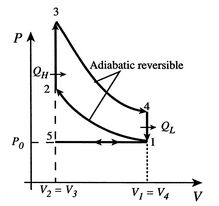
\includegraphics[height=80mm,width=100mm]{OttoIdeal.jpg}
  \caption{Otto Cycle-PV-diagram(Image courtesy \cite{ref14})}
  \label{fig:PV Diagram for Otto Cycle}
\end{figure}
\end{center}
\section{Introduction to Real Otto Cycle}
 The ideal cycle as the name suggests is ideal case i.e it involves lot of assumptions and thus does not occur in reality. Also the losses associated with each process are not being accounted in ideal cycle. The PV diagram of an real Otto Cycle (Figure 10) has similar shape as that of the ideal cycle (Figure 9), but the area (work) enclosed by the PV diagram of real cycle is always less than the area enclosed by PV diagram of ideal cycle. 
\newline Differences between ideal and real otto cycle are listed as follows:\newline
\textbf{1) } Major difference between the two cycles is that ideal cycle takes into account a simplified version of the intake and exhaust strokes. In the exhaust stroke, heat $Q_{out}$ is ejected to the environment, in a real engine, the gas leaves the engine and is replaced by a new mixture of air and fuel.

\textbf{2) } In Ideal cycle, Compression Stroke and Power Stroke expansion process involves no heat transfer i.e From $ 1\rightarrow2$ fuel air mixture is compressed adiabatically and From $ 3\rightarrow4$ the fuel-air mixture is expanded adiabatically. Whereas In real Otto cycle ,processes are polytropic and are not adiabatic.

\textbf{3) } Ideal cycles also assumes that no Pumping Work is involved in cycle i.e exhaust pressure is equal to inlet pressure. But In real cycles, due to difference between inlet pressure and exhaust pressure Pumping work is being arised and thus is equal to the difference between the work done in both strokes i.e exhaust and intake stroke.

\textbf{4) }Instantaneous heat addition is assumed in ideal cycle  during isochoric process from $ 2\rightarrow3$. In real engines the process is no longer isochoric which results  heat addition to be noninstantaneous and thus the peak pressure in real cycle is not at top dead centre, but just after it.

\textbf{5) } In Ideal cycle also involves complete combustion of fuel-air mixture which is not the case in real cycle.

\textbf{5) } Real cycle  takes into account losses due to friction whereas ideal cycle completely neglects frictional losses. 

\textbf{6) } Real Cycle also takes into account of other non-idealities such as early opening of exhaust valves during expansion stroke which results in a loss of work output (Blowdown Loss) and  losses due to the leakage of compressed gases through piston rings (Blow-by loss) .While ideal cycle assumes no Blow-by and Blowdown losses. 



\begin{figure}[!h]
  %\includegraphics[scale = 0.75]{13.jpg}\\[0.0 cm]
  \centering
    \vspace*{0 cm}
  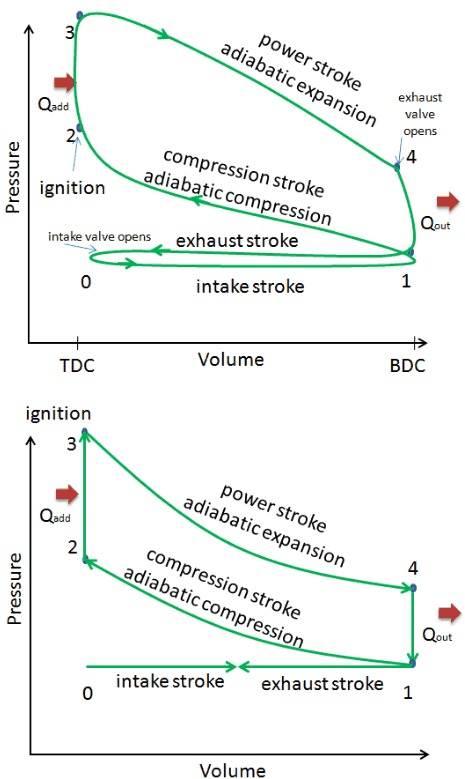
\includegraphics[width=100mm, height = 110mm]{idealNreal.jpeg}
    \caption{Real Otto Cycle(Image courtesy \cite{ref16} )}
  \label{fig:Real Otto Cycle}
\end{figure}

\pagebreak

\section{Efficiency of an ideal Otto cycle and Diesel Cycle}
The thermal efficiency expression for the otto cycle:
\textbf{\[  \eta = \frac{Work}{Heat \  Input} = \frac{Q_{add}-Q_{out}}{Q_{add}} = 1 - \frac{T_4 - T_1}{T_3 - T_2} = 1- {\big(\frac{V_2}{V_1}\big)}^{\gamma -1} \]}

it can be derived by following energy conservation principle i.e first law of thermodynamics. Here $Q_{out} = m C_v (T_4 - T_1)\  and\  Q_{add} = m C_v (T_3 - T_2) $ For futher simplification of expression the fact can be used that process from $ 1\rightarrow2$ and $ 3\rightarrow4$ are adiabatic ($\gamma = \frac{C_p}{C_v}$, Compression ratio $ r = \frac{V_1}{V_2}$ ).

\begin{figure}[!h]
  %\includegraphics[scale = 0.75]{13.jpg}\\[0.0 cm]
  \centering
    \vspace*{0 cm}
  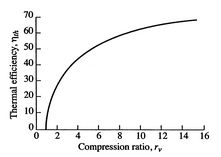
\includegraphics[height=80mm,width=100mm]{Efficiency.jpeg}
    \caption{Efficiency of Otto Cycle(Image courtesy \cite{ref14})}
  \label{fig:Otto Cycle Efficiency}
\end{figure}

The thermal efficiency expression for the diesel cycle:
\[ \eta = \frac{Work}{Heat \  Input} = \frac{Q_{add}-Q_{out}}{Q_{add}} = 1 - \frac{C_v(T_4 - T_1)}{C_p\ (T_3 - T_2)}\]

it can be derived by following energy conservation principle i.e first law of thermodynamics. Here $Q_{out} = m C_v (T_4 - T_1)\  and\  Q_{add} = m C_p (T_3 - T_2) $  

\subsection{Comparison of Otto Cycle with Diesel Cycle} 
In the Diesel cycle engines, internal combustion happens as only air is compressed with no fuel in it to very high pressure , which leads to rise in temperature of air. In Diesel Cycle the fuel is ignited by compression in the cylinder. As discussed above , The thermal efficiency of the Diesel cycle is dependent on Compression ratio (r)  and $ \gamma ( \frac{C_p}{C_v} ) $  and also on the cutoff ratio, $ r_c $, which is the ratio of the cylinder volume at the starting and ending of the combustion process.
The Otto cycle is more efficient than the Diesel cycle under the condition that the compression ratio is same \cite{ref17} . This is because in Diesel cycle, air can be compressed to higher compression ratio as it has no fuel in it and only air is compressed and thus there is no risk of spontaneous combustion of the fuel. whereas in Otto Cycle , the compression ratio is limited by a factor that is sufficient enough to prevent Knocking process in Otto Cycle engines which is basically uncontrolled combustion. 
With compression ratios in the range 8 to 11, thermal efficiency in ideal cycle is from 56 \% to 61\% .
Whereas practical Diesel engines in comparison to gasoline engines are 30 \% - 35\% more efficient due the fact that compression of only air takes place and the fuel is only introduced when it is required for ignition in the combustion chamber , thus there is no limit on compression ratio , so higher compression  ratios are used than in spark ignition engines.
\subsection{Comparison between two fuels -- Diesel and Petrol}
Though both the fuels are derived from the distillation of the crude oil, petrol is a low carbon content hydrocarbon in contrast with diesel which is a high carbon chain hydrocarbon. In the petrol engine which follows the spark ignited otto cycle, air and petrol are mixed (petrol is more volatile because of less carbons) which on compression follows with the spark ignition and hence the power cycle phase. Diesel is a heavy HC and is in liquid form. Thus during the compression, only the air is compressed in the diesel cycle. This compression creates very high temperature and pressure and then diesel drops are mixed which ignites without any sparking.\\
Diesel has more energy content per liter(36.9MJpL) as compared to petrol(33.7MJpL) hence is more efficient fuel, but due to a long chain hydrocarbon, it produces more \(CO_2\) emission as compared to the emission by petrol combustion.


\section{Contribution}

The workload pertaining to this term paper was divided evenly. The contribution of every member has been highlighted as follows:\\
\textbf{Gantavya Bhatt:} He was responsible for finding the template for the term paper and importing appropriate libraries used to write this latex. Sections and subsections in Classification of Engine based on mechanics, history of the engines and comparison between fuel -  diesel vs petrol were written by him. \\ 
\textbf{Hritik Bansal:} He was responsible for planning the flow of the term paper. The abstract and the section on Typical SI Engine Designs had been written by him. He had also worked on including the references in this term paper. \\
\textbf{Anubhav Bhatia:} The sections on Ideal Otto Cycle, Real Otto Cycle , Efficiency of an ideal Otto and Diesel Cycle  and Comparison between Otto and Diesel Cycle were written by him. He also contributed in finalizing the flow of the term paper. \\




%\bibliographystyle{plain}
%\bibliography{biblist}




\begin{thebibliography}{9}

\bibitem{fig1}
Figure: Four Stroke Cycle 
\\\texttt{https://www.researchgate.net/figure/Four-stroke-cycle-for-spark-ignition-engines-\\Wikipedia-2014\_fig15\_284950622}

\bibitem{ref2}
Four Stroke Cycle 
\\\texttt{http://courses.washington.edu/engr100/Section\_Wei/engine/UofWindsorManual/Four\%\\20Stroke\%20Cycle\%20Engines.htm}

\bibitem{ref3}
Compression Ratio 
\\\texttt{https://en.wikipedia.org/wiki/Compression\_ratio}

\bibitem{ref4}
Power Stroke in 4-Stroke Engine
\\\textt{https://www.grc.nasa.gov/www/k-12/airplane/engopt.html}

\bibitem{ref5}
Two Stroke Engine 
\\\texttt{Pg358-359, Fundamental of Thermal Sciences by Robert Turner and Yunus Cengel}


\bibitem{ref6}
Lecture2 on IC engines NPTEL 
\\\texttt{https://nptel.ac.in/courses/112103262/2}


\bibitem{ref7}
 Wankel Engine
\\\texttt{http://sites.psu.edu/christianhohlprofessionalportfolio/wp-content/uploads/sites\\/46027/2016/04/Wankel-Rotary-Engine-.pdf}

\bibitem{ref8}
 Mazda Wankel Engine
\\\texttt{https://www.foxnews.com/auto/mazda-rotary-engine-returning-in-2019}


\bibitem{ref9}
 Basic structure of a Piston
\\\texttt{https://en.wikipedia.org/wiki/Reciprocating\_engine\#/media/File:Four\_stroke\_engine\\\_diagram.jpg}


\bibitem{ref10}
 Section of a V-engine
\\\texttt{http://ffden-2.phys.uaf.edu/webproj/212\_spring\_2017/Christopher\_Williams\\/Christopher\_Williams/vs.html}

\bibitem{ref11}
A cad model for 6-cylinder inline engine\\
\texttt{https://grabcad.com/library/6-inline-engine-layout}

\bibitem{ref12}
A W16 engine of Buggati Veyron\\
\texttt{https://en.wikipedia.org/wiki/W16_engine}

\bibitem{ref13}
How a Rotary Engine Works\\
\texttt{https://www.youtube.com/watch?v=6BCgl2uumlI}

\bibitem{ref14}
 Otto Cycle process
\\\texttt{http://web.mit.edu/16.unified/www/FALL/thermodynamics/notes/node26.html}

\bibitem{ref15}
The very first newcomen engine\\
\texttt{https://en.wikipedia.org/wiki/Newcomen\_atmospheric\_engine}

\bibitem{ref16}
Ideal vs Actual Otto PV Diagram\\
\texttt{https://www.nuclear-power.net/nuclear-engineering/thermodynamics/thermodynamic-\\cycles/otto-cycle-otto-engine/theory-of-otto-cycle-gasoline-engine/}

\bibitem{ref17}
Gas power cycle \\
\texttt{https://nptel.ac.in/courses/112106133/Module\_4/8\_Comparison\_of\_Otto,\\Diesel,dual\_cycles.pdf}

\end{thebibliography}


\end{document}